%!TEX root = ../thesis.tex

\chapter{Grundlagen}
\label{chap:fundamentals}
\todo{Grundlagen einteilen und schreiben}
In diesem Kapitel werden die Grundlagen erläutert, die für das Verständnis dieser Arbeit wichtig sind. 

Zum einen werden in \prettyref{sec:darts} die Grundlagen des Dartsportes erläutert, auf deren Wesen die Idee dieser Abhandlung fußt. Dabei wird vom Dartboard bis zu den Darts und den allgemeinen Turnierregeln ein Überblick gegeben, um den Nutzen und die Motivation verständlicher zu machen.

Anschließend wird im \prettyref{sec:setup} das genutzte Testsetup dargestellt, welche für die praktische Implementierung genutzt wird.

Weiterhin werden grundlegende Informationen der Bildverarbeitung vermittelt im \prettyref{sec:basics}. Es wird ebenfalls ein Überblick über die verwendeten Bibliotheken zur Implementierung gegeben.
\section{Dartsport}
\label{sec:darts}
Der Dartsport hat im Jahr 1920 eine erste Standardisierung erhalten. Die 1924 gegründete "`National Dart Association"' hat diesen zum Standard ihrer Liga erklärt \autocite[5]{guide2013}. Diese Standardisierung findet sich in vielen heutigen Regelwerken der verschiedenen Verbänden wieder. Auch in der Sport- und Wettkampfordnung des Deutschen
Dart-Verband (DDV) \autocite{DartsRegel2016}. Aus dieser sind die Folgenden Erklärungen und Reglungen entnommen. 

Zunächst einmal zum Dartboard, das heutzutage genutzte Dartboard ist in Abbildung\prettyref{Fig:dartboard} zu sehen. In seiner heutigen Form wurde es zum Zeitpunkt der Standardisierung 1924 geschaffen. Die Größe des gesamten Boardes und der einzelnen Felder ist hierbei normiert und Standard. Wie in Abbildung \prettyref{Fig:dartboard} abzulesen. 

Heutzutage werden sogenannte Boards vom Typ "`Bristle"' verwendet. Dieser Name stammt vom englischen Wort für Bürste ab. Diese Board werden aus Sisal-Fasern gefertigt, welche in Aufprallrichtung der Pfeile aufgestellt sind, sodass die Pfeile sich zwischen die Fasern schieben können. \autocite[6]{dph2015}. Die Drähte, die die einzelnen Felder voneinander trennen werden "`Spider"' genannt.
\begin{figure}
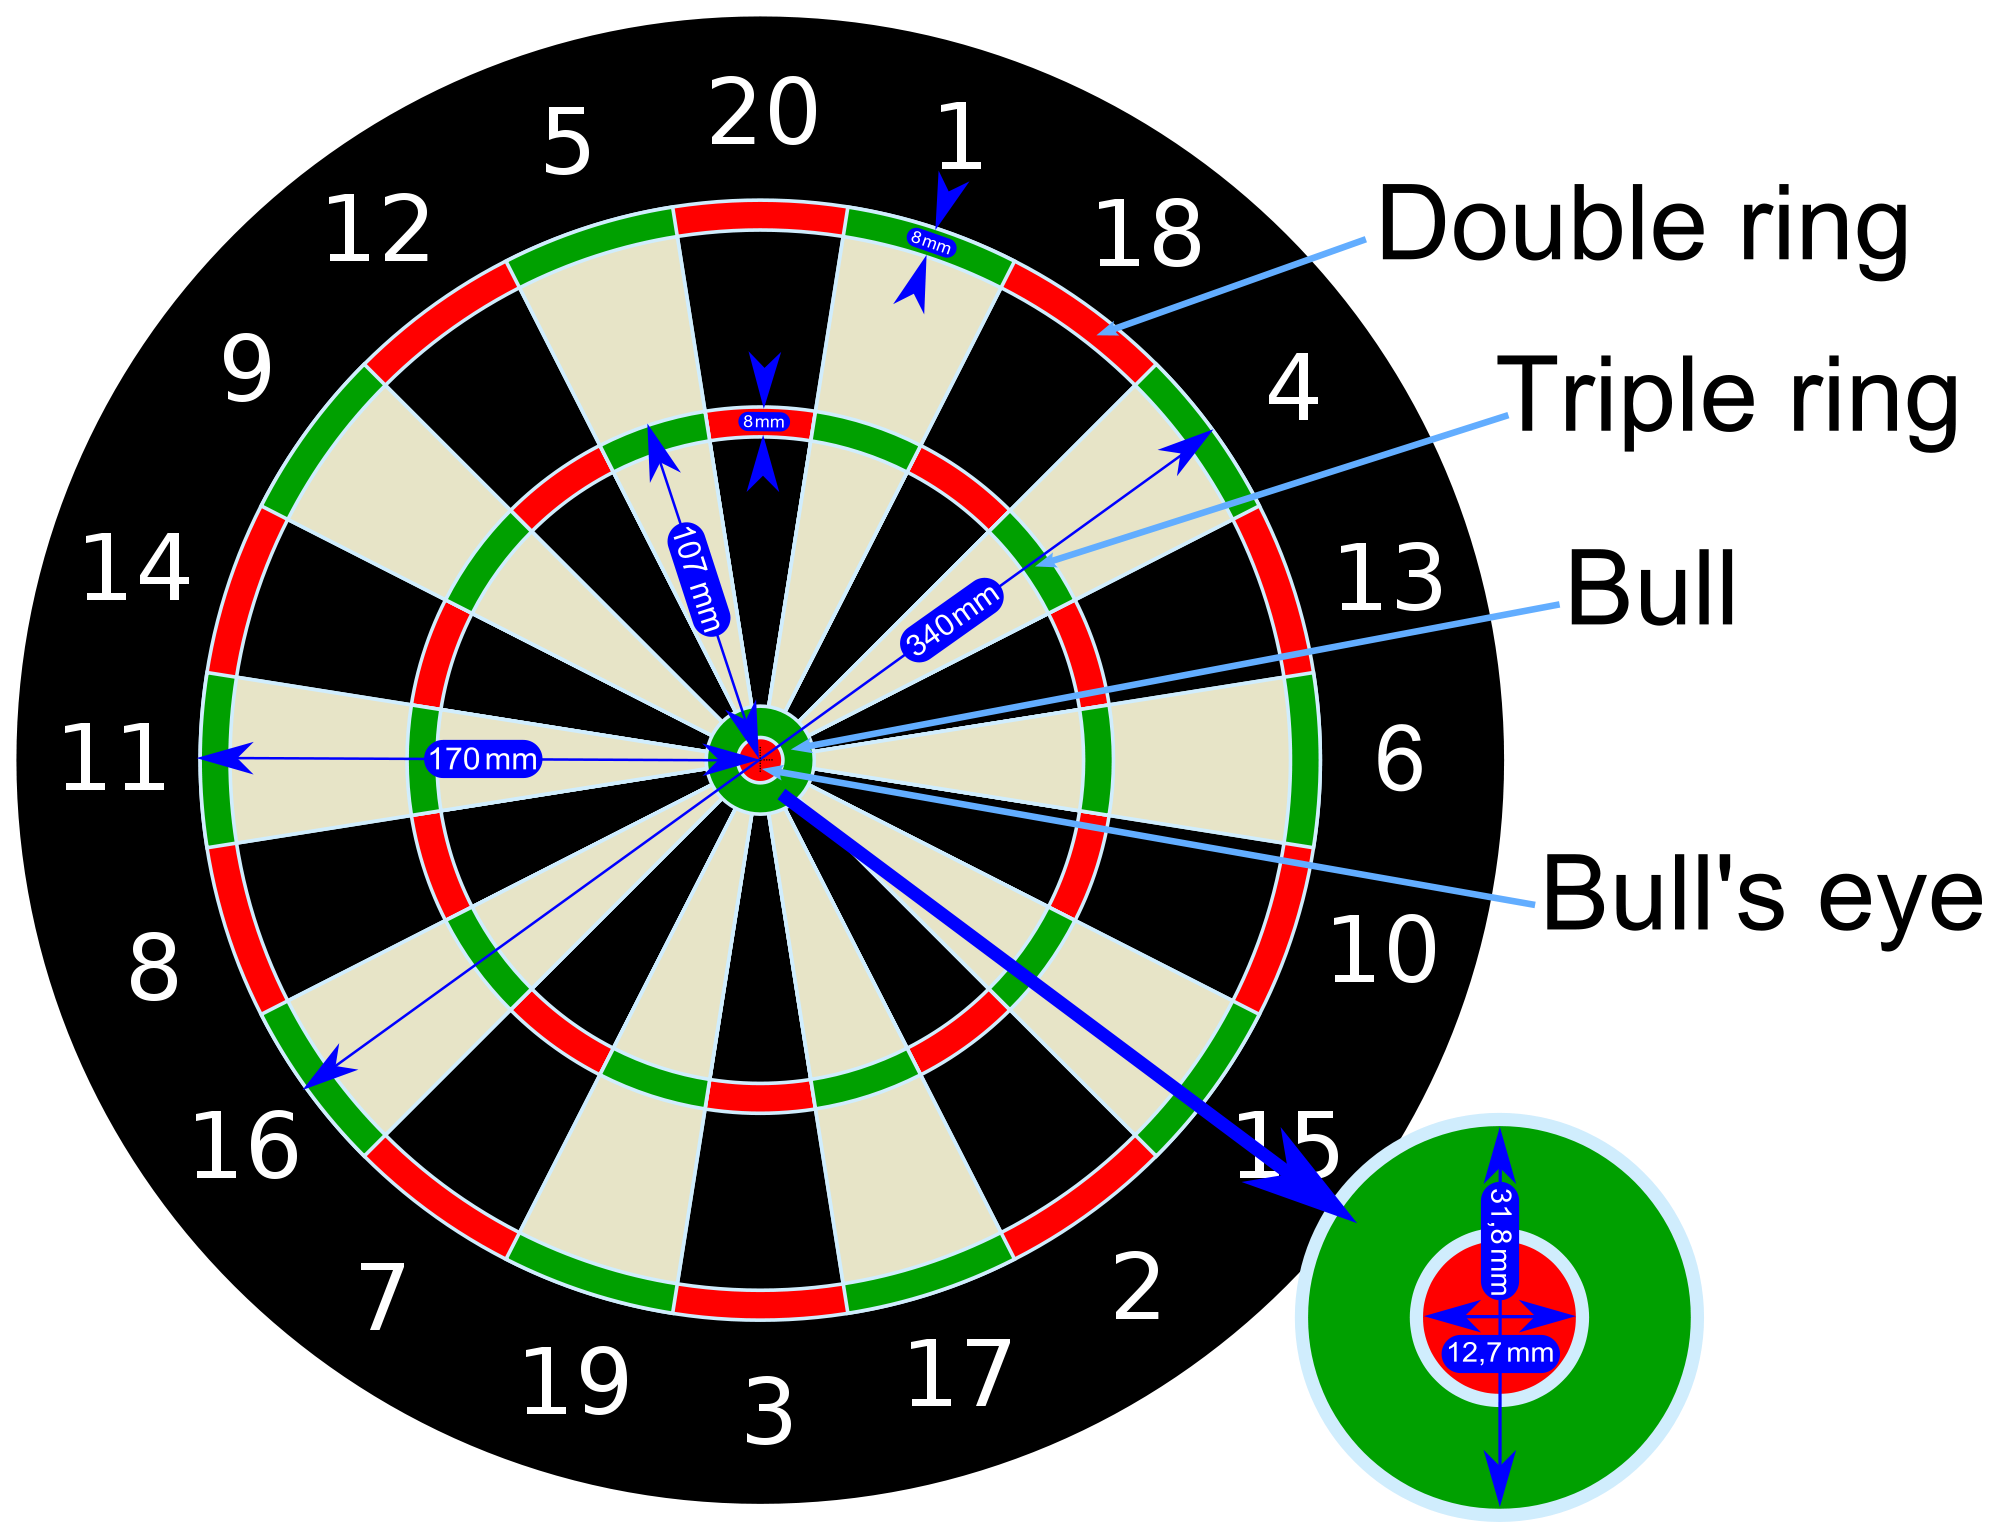
\includegraphics[width=\textwidth]{media/Dartboard_Abmessungen}\\
\caption{\textbf{Standardisiertes Dartboard\cite{Board2016}}
}
\label{Fig:dartboard}
\end{figure}

Die Anordnung der Ziffern ist hierbei von Oben im Uhrzeigersinn gelesen in der Folge 20-1-18-4-13-6-10-15-2-17-3-19-7-16-8-11-14-9-12-5. Diese wird als "`London Board"' bezeichnet. Hierbei wird der äußere 8mm breite Ring als "`Double Ring"' bezeichnet und und der innere als "`Triple Ring"' und verdreifacht die Punktzahl des Feldes. Der "`Bull"', der innere Bereich des Boards ist unterteilt in den grünen Teil genannt "`Half Bull"' and das "`Bullseye"', dieses zählen 25, bzw. 50 Punkte. 
Somit ist das "`Bullseye"' nicht, wie viele glauben, das Feld mit den meisten Punkten. Es gibt sogar gleich 4 Felder, die eine höhere Punktzahl erbringen, die Triple 20, 19, 18 und 17. Die Tripple 20 hat somit mit 60 Punkten die höchste zu erreichende Punktzahl. Im folgenden werden Triple Felder als "`TX"' bezeichnet, wobei X für die Ziffer des jeweiligen Feldes steht, zum Beispiel also T20. Eine weitere nennenswerte Schreibweise ist analog die für Doppelte Felder mit "`DX"'. 

\begin{figure}
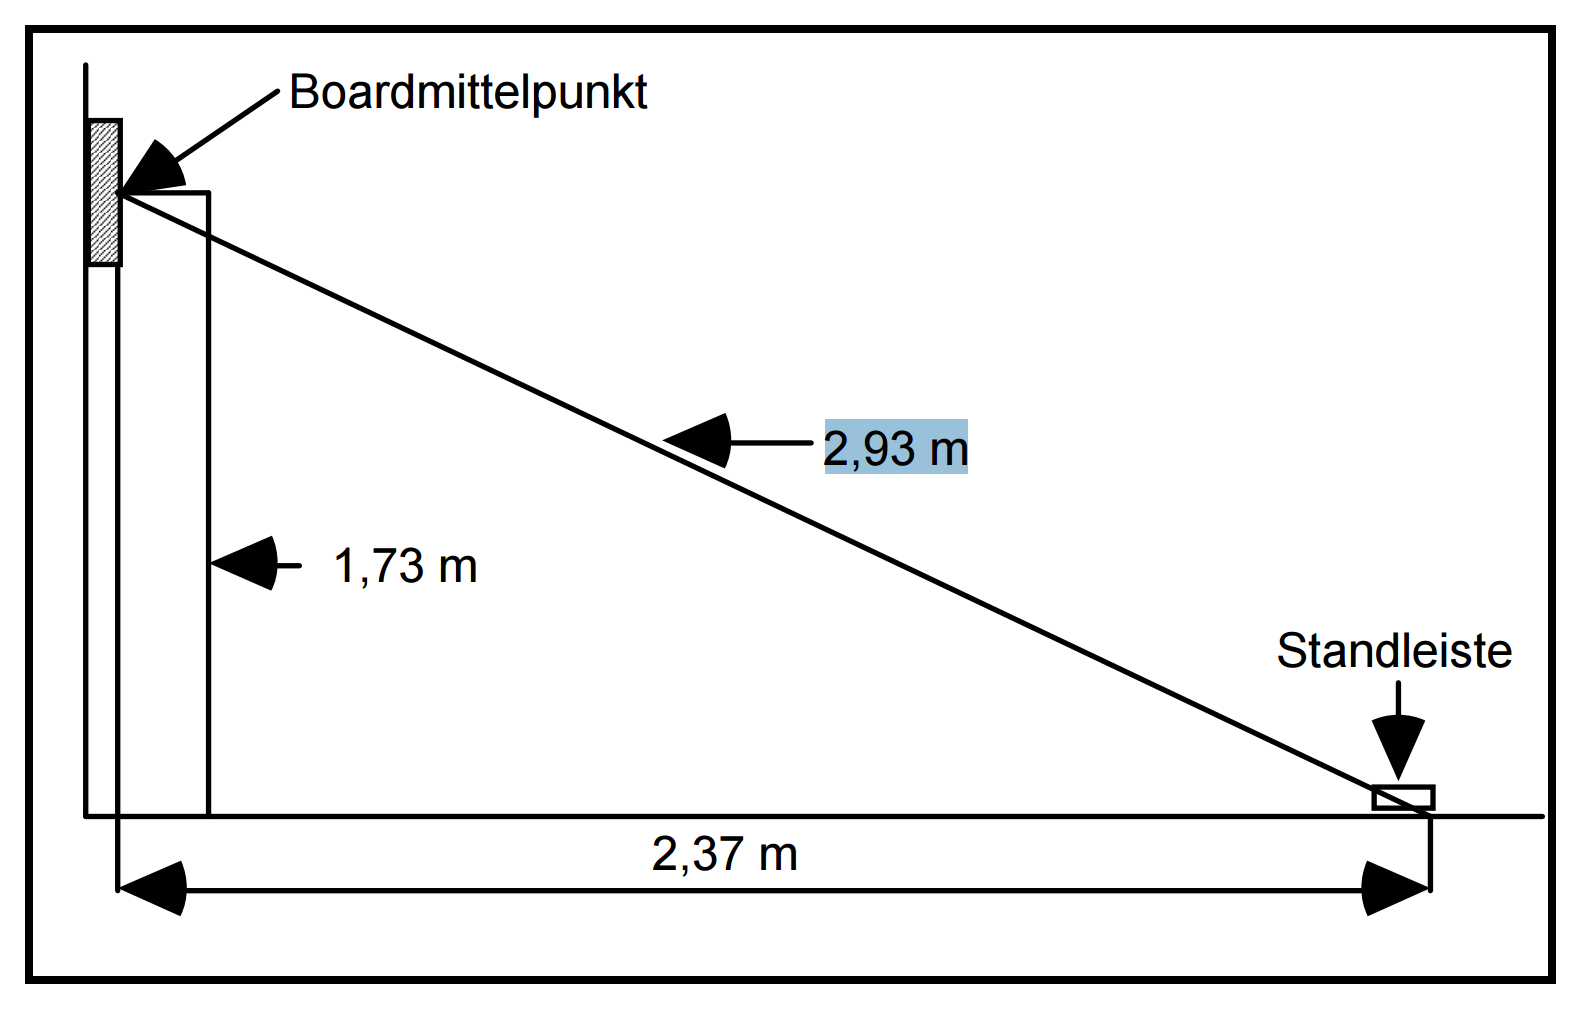
\includegraphics[width=\textwidth]{media/Dartsfield}\\
\caption{\textbf{Seitenansicht von Board und Standleiste 
\cite[8]{DartsRegel2016}}
}
\label{Fig:dartsetup}
\end{figure}


Das Board wird mit dem Mittelpunkt des "`Bullseyes"' auf eine Höhe von 1,73 gehängt, in der Weise, dass sich das Feld mit der 20 mittig oben befindet \autocite[6-8]{DartsRegel2016}. In Abbildung \prettyref{Fig:dartsetup} ist eine Seitenansicht einer Dartanlage nach dem Regelwerk des DDV zu sehen. Die Standleiste, oder "`Oche"' befindet sich hier in einer Entfernung von 2.37 zur Front-Seite des Boards. 

Als letzten Teil der Ausrüstung gilt es den Dart selbst zu beschreiben. Bei einem Dart, wie in Abbildung \prettyref{Fig:darts} zu sehen, sind grundsätzlich vier Hauptbestandteile zu unterscheiden:
\begin{enumerate}
    \item Point, Tip oder Spitze
    \item Barrel
    \addtocounter{enumi}{1}
    \item Shaft
    \addtocounter{enumi}{1}
    \item Flight
\end{enumerate}
\begin{figure}
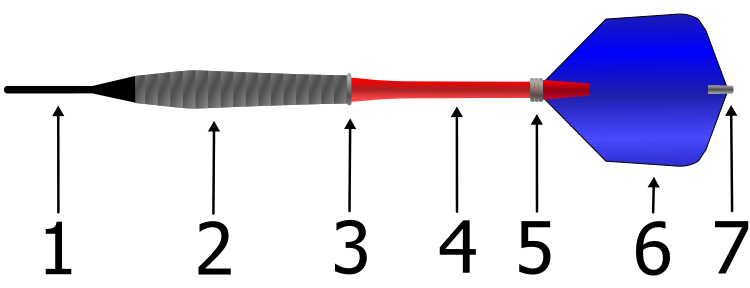
\includegraphics[width=\textwidth]{media/Dart}\\
\caption{\textbf{Aufbau eines Darts\cite{dart2006}}
}
\label{Fig:darts}
\end{figure}
Die weiteren Bestandteile sind optional und nicht zwingend notwendig für den Dart. 
\begin{enumerate}
	\addtocounter{enumi}{1}
	\addtocounter{enumi}{1}
    \item O-Ring, um den Shaft (4) fester im Barrel (2) zu befestigen
    \item Collar, dient dazu das Ende des Shafts zusammenzudrücken, um den Flight sicherer zu befestigen
    \addtocounter{enumi}{1}
    \item Flight Protector, dient dazu den Flight vor dem Auftreffen anderer Darts zu schützen

\end{enumerate}

Dart wird im Turniersport in zwei verschiedenen Modi gespielt, welche sich sehr ähneln. Zum einen 501 und zum anderen 301 mit "`Double Out"'.
Hierbei hat zunächst jeder Spieler einen Pool von genannter Punktzahl. Dieser wird mit jedem erzielten Punkt verringert. Ziel ist es als erster Spieler eine Punktzahl von 0 zu erreichen. Hierbei ist zu beachten, dass genau auf 0 heruntergespielt werden muss. Es ist also nicht möglich bei 10 verbleibenen Punkten eine höhere Punktzahl zu erwerfen. Des weiteren gilt für das Beenden, das dies mit einem Doppel-Feld erzielt werden muss. Somit müsste bei 10 verbleibenen Punkten eine D5 erzielt werden. Zusätzlich ist es auch möglich "`Bull Out"' zu erzielen, also nicht mit einem Doppelfeld abzuschlißen, sondern mit demm "`Bullseye"'. \todo{Quellen einfügen und nachschauen, wann genau Bull möglich ist, und was bei 1 verbleibenen Punkt passiert, bzw. wenn überworfen wird.}
Rechnerisch ist es bei 501 also möglich, mit 9 Darts zu beenden (3xT20, 3xT20, 2xT20+Bullseye) , der sogenannte "`Neun Darter"'.

Die bisher beschriebene Dart Variante ist wird als "`Steeldart"' bezeichnet, da die Darts in der Regel eine Stahlspitze besitzen und einen Metallshaft haben. Dem gegenüber gibt es noch das sogenannte "`Softdart"' \todo{Quelle einfügen}. Beim Softdart wird nicht mit Darts mit Stahlspitzen gespielt, sondern mit Kunststoffspitzen. Dem entsprechend



\section{Aufbau der Testumgebung}
\label{sec:setup}

\section{Grundlagen Bildverarbeitung}
\label{sec:basics}
Das Pinhole Camera Modell sieht wie folgt aus: \autocite{Zhang2000}.
\begin{figure}
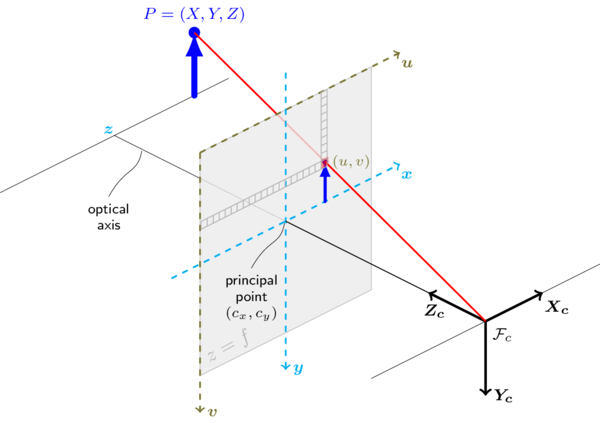
\includegraphics[scale =0.75]{media/pinhole_camera_model}\\
\caption{\textbf{Pinhole Camera Modell von.\autocite{OpencvCamera2016}}
}
\label{Fig:pinhole}
\end{figure}


\todo{pinhole Camera Modell erläutern}
\todo{opencv Benutzung erklären}
OpenCV ist eine \autocite[512--]{Medioni:2004:ETC:993884}

